\documentclass[hidelinks,english]{article}

\usepackage{graphicx}
\usepackage{grffile}
\usepackage[T1]{fontenc}
\usepackage{babel}
\usepackage{wrapfig}
\usepackage{hyperref}
\usepackage{geometry}
\usepackage{array}
\newcolumntype{L}[1]{>{\raggedright\let\newline\\\arraybackslash\hspace{0pt}}m{#1}}
\geometry{
	a4paper,
	total={170mm,257mm},
	left=20mm,
	top=20mm,
}

\date{\today}

\graphicspath{{Pictures/}}
\begin{document}	
	\begin{titlepage}
		\pagenumbering{gobble}
		\begin{figure}[!t]
			
\includegraphics[width=\linewidth]{up_logo.png}
		\end{figure}
		\vspace*{\stretch{1.2}}
		\begin{center}
			\huge{API User Manual\\}
			\huge{Mindmap PIM}\\
			\large{Client: IMINISYS}\\
			\vspace{10mm}
			\huge{Team: A-Cube-N}\\
		\end{center}
		\begin{center}
			\begin{tabular}{ c c c }
				Grobler, Arno & Lochner, Amy & Maree, Armand \\
				\texttt{14011396} & \texttt{14038600}& \texttt{12017800} \\				
			\end{tabular}
		\end{center}
		\begin{center}
			Department of Computer Science, University of Pretoria
		\end{center}
		\vspace*{\stretch{2.0}}
	\end{titlepage}
	\newpage
	\tableofcontents
	\newpage
	\pagenumbering{arabic}
	
	\section{Introduction} 
		\paragraph\indent
		This document will serve as a manual to external developers to interface with the Unclutter Polling API. This API will allow developers to more easily and more rapidly develop pollers for new platforms while at the same time hiding the technical details of the interaction between the pollers and the rest of the system.
		
	\section{Adding the Dependency}
		\paragraph\indent
		It is recommended that the poller is built with Gradle since the rest of the system also makes use of this, although it is not enforced.
		
		\paragraph\indent
		Figure \ref{gradledependency} shows the \emph{build.gradle} file. It indicates that the API must be added as a dependency.
		
		\begin{figure}[!h]
			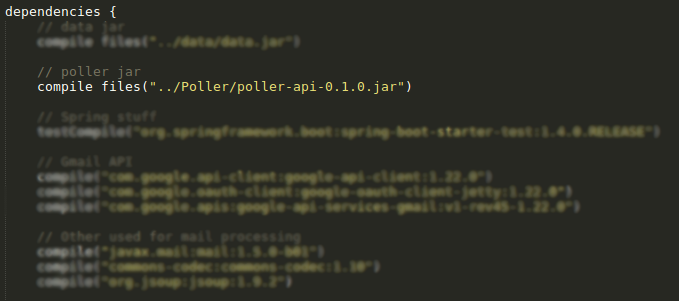
\includegraphics[width=\linewidth]{GradleDependency.png}
			\caption{Gradle Dependency}
			\label{gradledependency}
		\end{figure}
		 
	\section{Bean Setup}
		\paragraph\indent
		To simplify the processes it is recommended that you use Spring and allow it to manage the beans inside of the API. In order for Spring to do this, only a few simple steps need to be implemented.
		
		\paragraph{Firstly}\indent
		Let's assume your main Spring application class is called \emph{Application} saved in a file named \emph{Application.java}. In this class you need to create 3 beans (2 of which are optional, but recommended). These beans are:
		\begin{itemize}
			\item AuthCodeListener
			\item ItemRequestListener
			\item MessageBrokerFactory
		\end{itemize}
		
		\subsection{AuthCodeListener}
			\paragraph\indent
			The object contained in this bean should have one method that takes a single AuthCode object in as a parameter (see figure \ref{authcodelistenerparameter}). This is the method that should receive an authorization code and start the polling processes for the specified user. This bean is one of the optional ones, but if this object is not placed in a bean, then you will have to manage it manually.
		
			\begin{figure}[!h]
				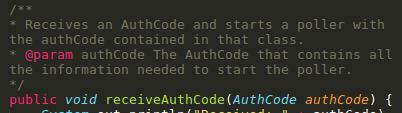
\includegraphics[width=\linewidth]{AuthCodeListenerParameter.png}
				\caption{AuthCodeListener Receiving Method}
				\label{authcodelistenerparameter}
			\end{figure}
			
		\subsection{ItemRequestListener}
			\paragraph\indent
			The object contained in this bean should have one method that takes a single ItemRequest object in as a parameter (see figure \ref{itemrequestlistenerparameter}). This is the method that should receive a request for an item, retrieve the specified item and send the item back (we will discuss this in section \ref{itemresponsesend}) This bean is one of the optional ones, but if this object is not placed in a bean, then you will have to manage it manually.
			
			\begin{figure}[!h]
				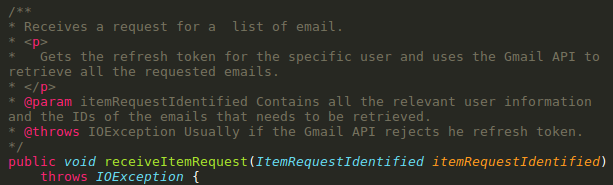
\includegraphics[width=\linewidth]{ItemRequestListenerParameter.png}
				\caption{ItemRequestListener Receiving Method}
				\label{itemrequestlistenerparameter}
			\end{figure}
			
		\subsection{MessageBrokerFactory}
			\paragraph\indent
			The MessageBrokerFactory is the core of the API. It contains all the complicated configuration for the Spring beans that interact with the rest of the system so that you do not have do it manually. Creating this bean requires the following steps (code is provided in figure \ref{messagebrokerfactorybean}):
			\begin{itemize}
				\item Create a \emph{PollingConfiguration} object and in the constructor provide the following in this order:
					\begin{itemize}
						\item Name of platform (like "gmail" or "facebook"). A string that contains lowercase letters.
						\item The AuthCodeListener object created in the bean in the previous section.
						\item A string of the name of the method in AuthCodeListener that will be receiving the AuthCode object.
						\item The ItemRequestListener object created in the bean in the previous section.
						\item A string of the name of the method in ItemRequestListener that will be receiving the ItemRequest object.
					\end{itemize}
				\item Create a new \emph{MessageBrokerFactory} and in the constructor parameter pass in the \emph{PollingConfiguration} object you just created.
				\item Since the factory is now ready to produce \emph{MessageBroker}s you can pass a instance of this class (created by the factory) to each listener.
			\end{itemize}
			
		\begin{figure}[!h]
			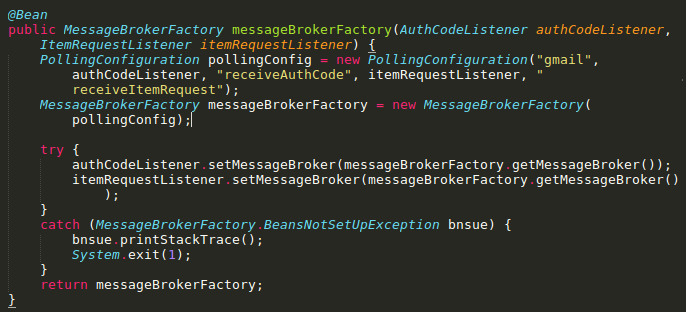
\includegraphics[width=\linewidth]{MessageBrokerFactoryBean.png}
			\caption{MessageBrokerFactory Bean Example}
			\label{messagebrokerfactorybean}
		\end{figure}
			
	\section{Sending RawData Objects}
		\paragraph\indent
		The poller will send \emph{RawData} objects via a \emph{MessageBroker} object that is created by the \emph{MessageBrokerFactory} that is set up in the previous section. There are two kinds of RawData. The first is called priority RawData, i.e. it needs to be processed rapidly by the rest of the system, and secondly standard non-priority \emph{RawData}, i.e. it does not have to be processed immediately.
		
		\paragraph\indent
		When a poller has received a new item (like an email or post), the poller can send this item (in the form of a \emph{RawData} object) to the rest of the system for processing and persistence via two methods contained in the \emph{MessageBroker} class. Priority \emph{RawData} objects can be sent with the \emph{sendPriorityRawData} method and non-priority \emph{RawData} objects can be sent with the \emph{sendRawData} method. See figure \ref{sendrawdata}.
		
		\begin{figure}[!h]
			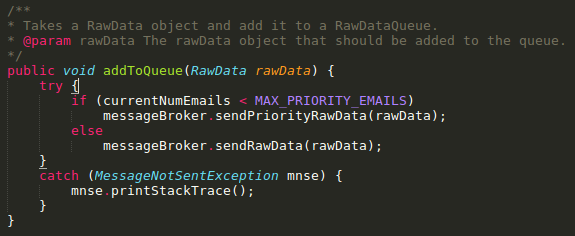
\includegraphics[width=\linewidth]{SendRawData.png}
			\caption{Send RawData}
			\label{sendrawdata}
		\end{figure}
		
		\section{Sending ItemResponse Objects}\label{itemresponsesend}
		\paragraph\indent
		So once you have received an item request and retrieved the item from the specific external platform, it is time to send it back to the requesting service. This is as simple as calling the \emph{sendItemResponse} method of the \emph{MessageBroker} class. See figure \ref{senditemresponse}.
		
		\begin{figure}[!h]
			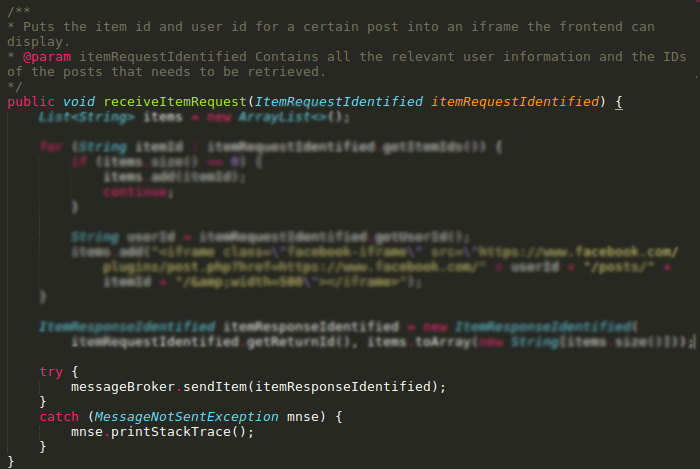
\includegraphics[width=\linewidth]{SendItemResponse.png}
			\caption{Send RawData}
			\label{senditemresponse}
		\end{figure}
		
	\section{Conclusion}
		\paragraph\indent
		As seen here, the API hides a lot of the complicated internal working from the poller developer which should speed up and simplify the development of new pollers. Should this guide not be sufficient for you, you are more than welcome to look at the JavaDoc documentation provided. The JavaDoc explains in great detail the purpose of each method, parameter and class.  
				
\end{document}
